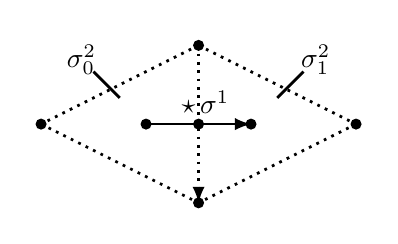
\begin{tikzpicture}[>=latex]
  % Coords
  \coordinate (V0) at (2,0);
  \coordinate (V1) at (2,2);
  \coordinate (V2) at (0,1);
  \coordinate (V3) at (4,1);
  % Arrows\tilde{\sigma}
  \draw[line width=1pt, ->, style=dotted]
    (V1) -- (V0);
  \draw[line width=1pt, style=dotted]
    (V1) --  (V2);
  \draw[line width=1pt, style=dotted]
    (V2) -- (V0);
  \draw[line width=1pt, style=dotted]
    (V1) --  (V3);
  \draw[line width=1pt, style=dotted]
    (V3) -- (V0);
  % Points
  \fill (V0) circle (2pt);
  \fill (V1) circle (2pt);
  \fill (V2) circle (2pt);
  \fill (V3) circle (2pt);
  %circumcenter
  \coordinate (CC0) at (1.333,1);
  \coordinate (CC1) at (2.666,1);
  \coordinate (CCC) at (2,1);
  \fill (CC0) circle (2pt);
  \fill (CC1) circle (2pt);
  \fill (CCC) circle (2pt);
  \draw[line width=1pt, ->]
    (CC0) -- node[above] {\( \,\,\,\star\,\sigma^{1} \)} (CC1);
  % nodes
  \draw[line width=1pt]
    (0.666,1.666) -- node[above left] {\( \sigma^{2}_{0} \)} (1,1.333);
  \draw[line width=1pt]
    (3.333,1.666) -- node[above right] {\( \sigma^{2}_{1} \)} (3,1.333);
	
\useasboundingbox ([shift={(1mm,1mm)}]current bounding box.north east) rectangle ([shift={(-1mm,-1mm)}]current bounding box.south west);
\end{tikzpicture}

